\documentclass[aspectratio=169,12pt]{beamer}

% Theme and colours
\usetheme{Madrid}
\usecolortheme{whale}
\setbeamertemplate{navigation symbols}{}
\setbeamertemplate{footline}[frame number]
\setbeamercolor{frametitle}{bg=structure.fg!15!white}

% Packages
\usepackage[T1]{fontenc}
\usepackage[utf8]{inputenc}
\usepackage{graphicx}
\usepackage{booktabs}
\usepackage{tikz}
\usepackage{lmodern}

% Metadata
\title{\textbf{Intelligent Retail Ecosystem}}
\subtitle{Ambient Intelligence -- In-Store Navigation \& Product Finding}
\author{David Correia \quad Gon\c{c}alo Oliveira \quad Pedro Duarte}
\institute{IST -- Alameda G11}
\date{}

% ═══════════════════════════════════════════════════════════════════
\begin{document}

% ── SLIDE 1: Title ────────────────────────────────────────────────
\begin{frame}
\titlepage
\end{frame}

% ── SLIDE 2: Live Demo Opening ────────────────────────────────────
\begin{frame}{Live Demonstration}
\begin{center}
\Large\textbf{``Find me lobster.''}\\[1.5em]
\normalsize
\textit{Watch the system locate a user in real time,\\
compute the optimal path, and guide them to the shelf\\
with turn-by-turn voice instructions.}\\[2em]
\textbf{[LIVE DEMO ON PHONE]}
\end{center}
\end{frame}

% ── SLIDE 3: The Problem ──────────────────────────────────────────
\begin{frame}{The Problem: Search Friction}
\begin{columns}[T]
\begin{column}{0.55\textwidth}
\textbf{The Information-Location Gap}
\begin{itemize}
    \item Digital inventories know \textit{what} is in stock
    \item They fail to tell shoppers \textit{exactly where} it is
    \item Shoppers face ``search fatigue'' in large layouts
    \item Staff waste time on manual stock-location audits
\end{itemize}
\vspace{1em}
\textbf{Scale of the problem:}\\
Average IKEA visit: 2.5 hours\\
Up to 40\% of time spent \textit{searching}, not shopping
\end{column}
\begin{column}{0.4\textwidth}
\begin{block}{Who is affected?}
\begin{description}
    \item[Shoppers] Want items fast
    \item[Staff] Need efficient picking
    \item[Managers] Seek higher conversion
\end{description}
\end{block}
\end{column}
\end{columns}
\end{frame}

% ── SLIDE 4: Value Proposition ────────────────────────────────────
\begin{frame}{Value Proposition}
\begin{center}
\Large\textit{``Transform any store into an interactive assistant.''}
\end{center}
\vspace{0.5em}
\begin{columns}[T]
\begin{column}{0.32\textwidth}
\begin{block}{\centering Efficiency}
\centering
Reduces ``time-to-item''\\
Optimised multi-product routes\\
Faster shopper throughput
\end{block}
\end{column}
\begin{column}{0.32\textwidth}
\begin{block}{\centering Accuracy}
\centering
1--1.5\,m positioning\\
Shelf-level guidance\\
Real-time path updates
\end{block}
\end{column}
\begin{column}{0.32\textwidth}
\begin{block}{\centering Accessibility}
\centering
Voice search (hands-free)\\
TTS turn-by-turn audio\\
Barrier-free navigation
\end{block}
\end{column}
\end{columns}
\vspace{1em}
\begin{center}
\textbf{No specialised hardware needed} -- works with any Android phone + low-cost ESP32 boards
\end{center}
\end{frame}

% ── SLIDE 5: Solution Overview ────────────────────────────────────
\begin{frame}{How It Works}
\begin{enumerate}
    \item \textbf{Search} -- Voice or text: ``Find lobster''
    \begin{itemize}
        \item Native Android speech recognition + fuzzy text matching
    \end{itemize}
    \item \textbf{Locate} -- System knows where you are
    \begin{itemize}
        \item 3 ESP32 gateways pick up your phone's BLE signal
        \item Phone IMU (steps + heading) fused via Kalman filter
    \end{itemize}
    \item \textbf{Navigate} -- Optimal path to the product
    \begin{itemize}
        \item A* pathfinding on a 0.25\,m grid with obstacle avoidance
        \item Multi-product queue: nearest-neighbour TSP + 2-opt
    \end{itemize}
    \item \textbf{Guide} -- Turn-by-turn voice directions
    \begin{itemize}
        \item TTS at each waypoint: ``Turn left'', ``Almost there''
        \item Arrival: ``You have arrived. Lobster is on the upper shelf.''
    \end{itemize}
\end{enumerate}
\end{frame}

% ── SLIDE 6: Architecture ─────────────────────────────────────────
\begin{frame}{System Architecture}
\begin{center}
% Replace with im1.png if available
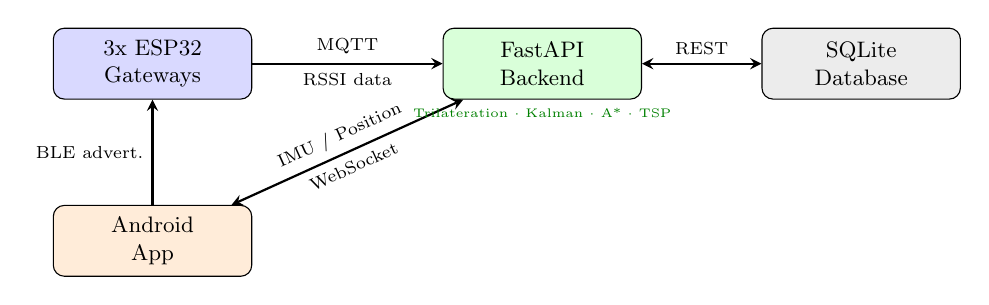
\begin{tikzpicture}[
    box/.style={draw, rounded corners, minimum width=2.8cm, minimum height=1cm, align=center, font=\small},
    arrow/.style={->, thick, >=stealth},
    scale=0.9, every node/.style={scale=0.9}
]
% ESP32 layer
\node[box, fill=blue!15] (esp) at (0,0) {3x ESP32\\Gateways};
% Backend
\node[box, fill=green!15] (back) at (5.5,0) {FastAPI\\Backend};
% Phone
\node[box, fill=orange!15] (phone) at (0,-2.5) {Android\\App};
% DB
\node[box, fill=gray!15] (db) at (10,0) {SQLite\\Database};

% Arrows
\draw[arrow] (esp) -- node[above, font=\scriptsize] {MQTT} node[below, font=\scriptsize] {RSSI data} (back);
\draw[arrow] (phone) -- node[left, font=\scriptsize] {BLE advert.} (esp);
\draw[arrow, <->] (phone) -- node[below, font=\scriptsize, sloped] {WebSocket} node[above, font=\scriptsize, sloped] {IMU / Position} (back);
\draw[arrow, <->] (back) -- node[above, font=\scriptsize] {REST} (db);

% Processing labels inside backend
\node[font=\tiny, text=green!50!black] at (5.5, -0.7) {Trilateration $\cdot$ Kalman $\cdot$ A* $\cdot$ TSP};
\end{tikzpicture}
\end{center}
\vspace{0.5em}
\begin{columns}[T]
\begin{column}{0.32\textwidth}
\centering\textbf{Edge Layer}\\
\small ESP32 scan BLE, filter by \texttt{IRE-} prefix, publish RSSI via MQTT
\end{column}
\begin{column}{0.32\textwidth}
\centering\textbf{Processing Layer}\\
\small Kalman fusion $[x,y,v_x,v_y]$, A* pathfinding, route optimisation
\end{column}
\begin{column}{0.32\textwidth}
\centering\textbf{Client Layer}\\
\small Kotlin + WebView, BLE advertising, IMU streaming at 10\,Hz
\end{column}
\end{columns}
\end{frame}

% ── SLIDE 7: Technical Deep Dive ──────────────────────────────────
\begin{frame}{Technical Highlights}
\begin{columns}[T]
\begin{column}{0.48\textwidth}
\textbf{Hybrid Localisation}
\begin{itemize}
    \item BLE trilateration (weighted least-squares)
    \item RSSI smoothed with EMA ($\alpha = 0.65$)
    \item Kalman predict: PDR (steps + heading)
    \item Kalman update: BLE position
    \item Process noise scales with $\Delta t$
    \item Dynamic R based on signal strength
\end{itemize}
\vspace{0.5em}
\textbf{Result:} 3.5\,m error $\rightarrow$ 1--1.5\,m
\end{column}
\begin{column}{0.48\textwidth}
\textbf{Navigation Engine}
\begin{itemize}
    \item A* on 0.25\,m grid (40x20 cells)
    \item Shelf obstacles with margin buffer
    \item Douglas-Peucker path simplification
    \item NN-TSP + 2-opt for multi-product
    \item TTS at each waypoint (2\,s cooldown)
    \item Arrival within 1.8\,m triggers shelf-level announcement
\end{itemize}
\vspace{0.5em}
\textbf{Latency:} 1,490\,ms end-to-end
\end{column}
\end{columns}
\end{frame}

% ── SLIDE 8: Technology Stack ─────────────────────────────────────
\begin{frame}{Technology Stack}
\begin{table}
\centering
\small
\begin{tabular}{@{}ll@{}}
\toprule
\textbf{Layer} & \textbf{Technology} \\
\midrule
Mobile App      & Kotlin, Android WebView, BLE Advertiser \\
Frontend        & React 18, Vite, Canvas 2D \\
Backend         & Python 3.11, FastAPI, SQLAlchemy, SQLite \\
Localisation    & BLE trilateration, Kalman filter, PDR \\
Pathfinding     & A* + Douglas-Peucker, 2-opt TSP \\
Communication   & MQTT (Mosquitto), WebSockets \\
Voice           & Android SpeechRecognizer, SpeechSynthesis TTS \\
IoT Hardware    & 3x ESP32-WROOM, BLE 4.0+ \\
\bottomrule
\end{tabular}
\end{table}
\vspace{0.5em}
\begin{center}
\textbf{Total hardware cost:} $\sim$\texteuro 15 (3x ESP32 at \texteuro 5 each) + any Android phone
\end{center}
\end{frame}

% ── SLIDE 9: Results ──────────────────────────────────────────────
\begin{frame}{Results: Requirements Satisfaction}
\begin{table}
\centering
\small
\begin{tabular}{@{}lll@{}}
\toprule
\textbf{Requirement} & \textbf{Status} & \textbf{Key Metric} \\
\midrule
R1.1 Precision ($<$1.5\,m)  & Satisfied & 1--1.5\,m with IMU fusion \\
R1.2 Stability              & Partially & Jumps reduced, not eliminated \\
R1.3 Latency ($<$1.5\,s)    & Satisfied & 1,490\,ms measured \\
R2.1 Voice + Text Search    & Satisfied & Native speech + fuzzy match \\
R2.2 Route Optimisation     & Satisfied & TSP + 2-opt recalculation \\
R2.3 Wayfinding             & Satisfied & A* + TTS turn-by-turn \\
R2.4 Micro-Navigation       & Partially & TTS shelf-level (no CV) \\
R3.1 Android                & Satisfied & Android 12+, tested on A32 \\
\bottomrule
\end{tabular}
\end{table}
\vspace{0.5em}
\textbf{6 of 8 requirements fully satisfied}, 2 partially satisfied with clear paths to improvement.
\end{frame}

% ── SLIDE 10: Demo Backup Plan ────────────────────────────────────
\begin{frame}{Backup Demo Plan}
\textit{If the live demo encounters issues, switch to pre-recorded video:}
\vspace{0.5em}
\begin{enumerate}
    \item \textbf{App launch} -- Show the store map with user position dot (10\,s)
    \item \textbf{Voice search} -- Say ``Find lobster'', show results (10\,s)
    \item \textbf{Add to queue} -- Add 3 products, show optimised route (10\,s)
    \item \textbf{Navigation} -- Walk toward first shelf, hear TTS directions (20\,s)
    \item \textbf{Arrival} -- Reach shelf, hear ``You have arrived'' + shelf level (10\,s)
    \item \textbf{Admin panel} -- Show shelf/product management interface (10\,s)
\end{enumerate}
\vspace{0.5em}
\textbf{Total video length:} $\sim$70 seconds\\
\textbf{Recording device:} Screen record on the Samsung Galaxy A32
\end{frame}

% ── SLIDE 11: Future Work & Closing ──────────────────────────────
\begin{frame}{Future Improvements \& Closing}
\begin{columns}[T]
\begin{column}{0.48\textwidth}
\textbf{Next Steps}
\begin{itemize}
    \item Add more ESP32 gateways for tighter triangulation
    \item Optimise beacon scan cycle ($<$1\,s)
    \item Integrate computer vision for on-shelf product identification
    \item Cross-platform support (iOS)
    \item Analytics dashboard for store managers
\end{itemize}
\end{column}
\begin{column}{0.48\textwidth}
\textbf{What We Built}
\begin{itemize}
    \item A complete indoor navigation system
    \item 1--1.5\,m accuracy with \texteuro 15 of hardware
    \item Voice-guided, hands-free shopping
    \item Multi-product route optimisation
    \item Admin panel for staff
    \item 1.49\,s end-to-end latency
\end{itemize}
\end{column}
\end{columns}
\vspace{1.5em}
\begin{center}
\Large\textbf{We turned a store into an intelligent assistant.}\\[0.5em]
\normalsize Thank you. Questions?
\end{center}
\end{frame}

\end{document}
